% Figure F2, panel A: the state patch keeps the visible text fixed while
% swapping the stored value. Same visual encoding as d_protocol.tex:
% solid box = visible text, dashed box = hidden state, green = intervention.
\documentclass[tikz]{standalone}
\usetikzlibrary{positioning,arrows.meta}
\definecolor{okgreen}{HTML}{009E73}
\definecolor{okverm}{HTML}{D55E00}
\begin{document}
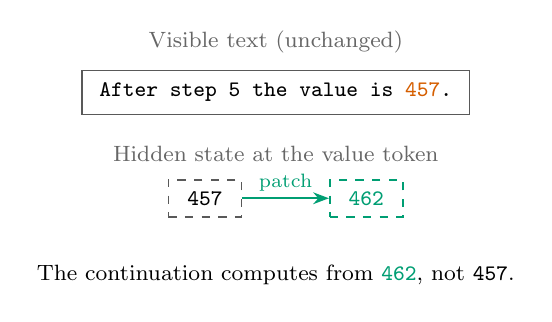
\begin{tikzpicture}[
  font=\footnotesize,
  span/.style={draw=black!65, line width=0.5pt, inner xsep=2.2mm,
               inner ysep=1.6mm, align=center},
  hidden/.style={dashed, line width=0.6pt, inner xsep=2.4mm,
                 inner ysep=1.5mm, align=center},
  lbl/.style={inner sep=1pt, color=black!60},
  arr/.style={-{Stealth[length=2.0mm]}, line width=0.7pt},
]
\node[lbl] (t1) {Visible text (unchanged)};
\node[span, below=1.8mm of t1] (vt)
  {\ttfamily After step 5 the value is \textcolor{okverm}{457}.};
\node[lbl, below=3.5mm of vt] (t2) {Hidden state at the value token};
\node[hidden, draw=black!65, below=1.8mm of t2, xshift=-9mm] (s1)
  {\ttfamily 457};
\node[hidden, draw=okgreen, right=11mm of s1, text=okgreen] (s2)
  {\ttfamily 462};
\draw[arr, okgreen] (s1) -- node[above, inner sep=2pt,
  font=\scriptsize, text=okgreen] {patch} (s2);
\node[below=4.5mm of t2.south, anchor=north, yshift=-7mm, align=center]
  (out) {The continuation computes from
  \textcolor{okgreen}{\ttfamily 462}, not {\ttfamily 457}.};
\end{tikzpicture}
\end{document}
